La primer etapa de experimentación consistió en contrastar empíricamente la cota de complejidad temporal obtenida de forma teórica para el algoritmo propuesto. Dado que la función de ordenamiento pertenece a la librería de C++ y a que su análisis de peor caso es altamente complejo, medimos el rendimiento de nuestra implementación sobre instancias generadas pseudo-aleatoriamente y no en instancias de peor caso. Y luego Esto limita la experimentación a un análisis de caso promedio.

Medimos el tiempo de ejecución al resolver instancias de entre 1 y 10000 camiones, según las consideraciones de la sección \ref{consideraciones-mediciones}, permitiendo graficar el costo temporal de la implementación en función del tamaño de entrada $T(n)$. En la figura (\ref{fig:problema1-aleatoria-10000}) se observan los resultados obtenidos.

\begin{center}
  \begin{figure}[H]
    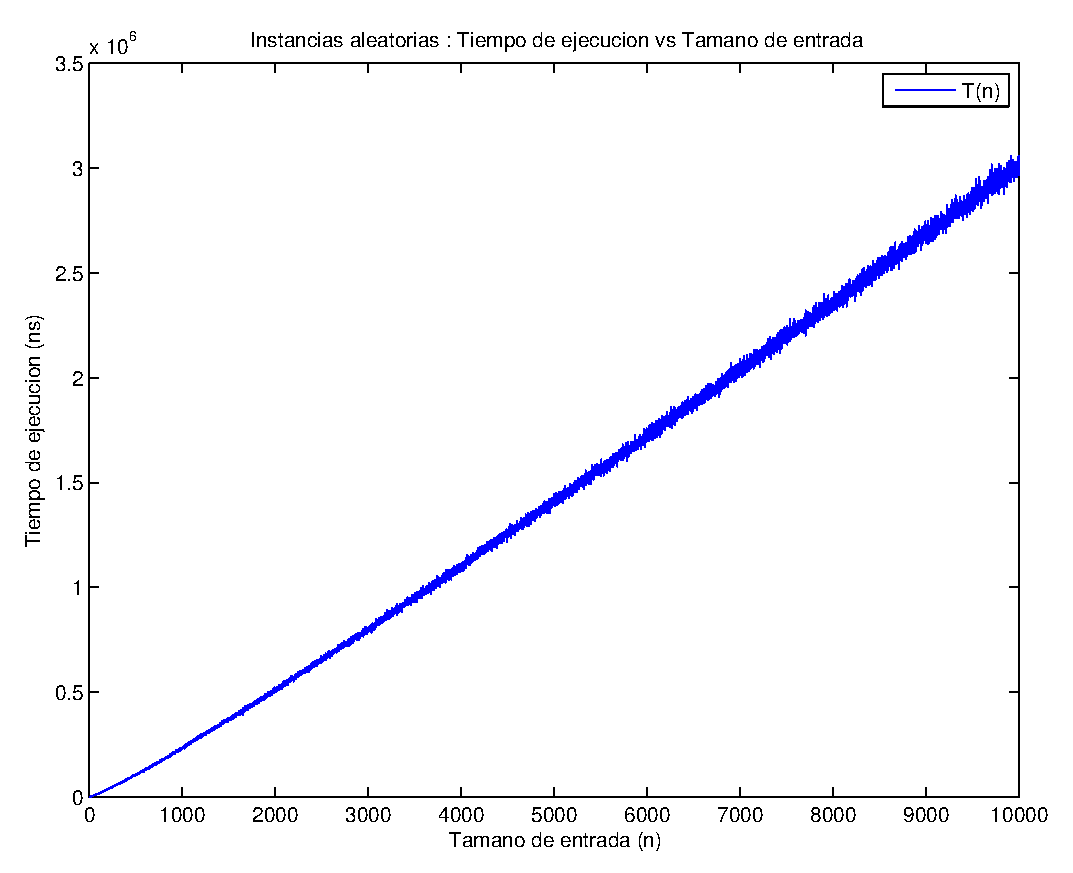
\includegraphics[width=0.5\linewidth]{problema1/graficos/problema1_aleatoria_10000.eps}
    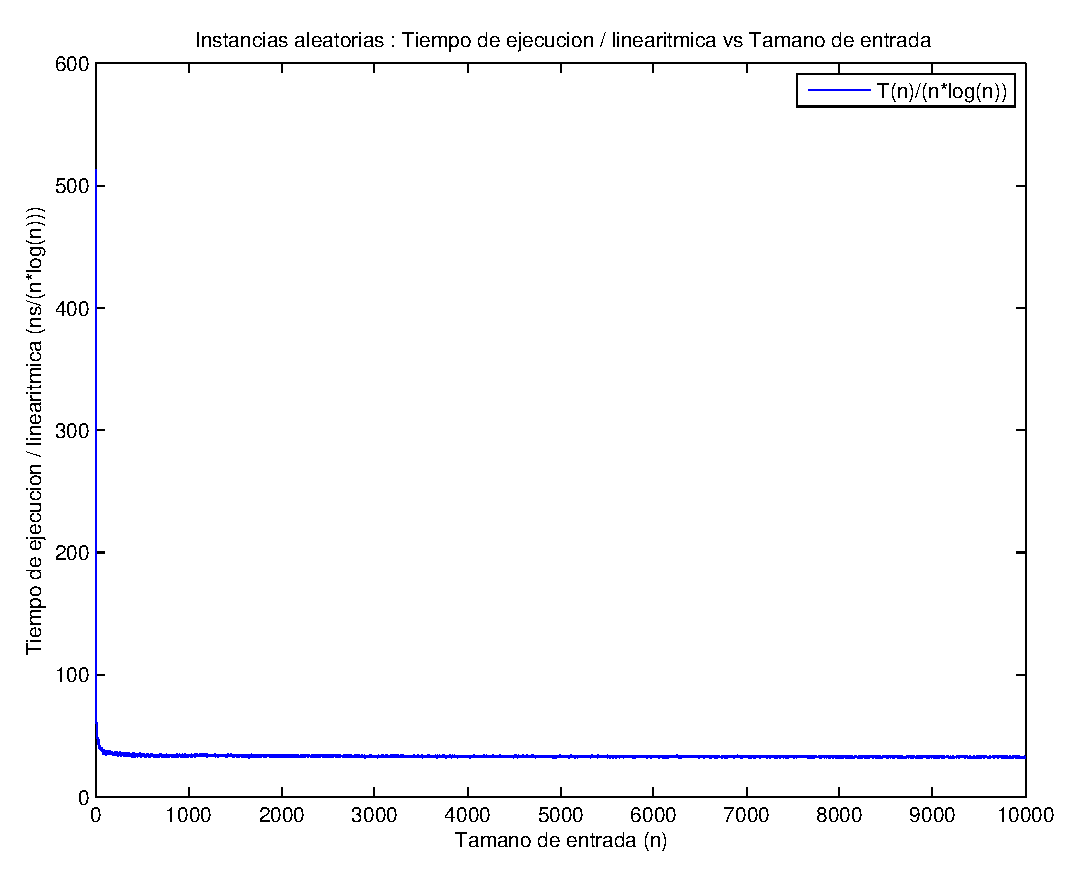
\includegraphics[width=0.5\linewidth]{problema1/graficos/problema1_aleatoria_10000_div_nlogn.eps}
    \caption{Instancias aleatorias, $1 \leq n \leq 10000$. Izquierda: $T(n)$ vs $n$. Derecha: $T(n) / (n * log(n))$ vs $n$.}
    \label{fig:problema1-aleatoria-10000}
  \end{figure}
\end{center}

Además de presentar los datos según fueron medidos, incluímos un gráfico donde se muestra el comportamiento del costo temporal para instancias de tamaño $n$ dividido $n * log(n)$. Esto permite visualizar la tendencia asintótica del cociente $T(n) / (n * log(n))$, que en este caso se aproxima a una constante cercana al valor $40$, sugiriendo dentro del marco de mediciones que $T(n)$ tiende a un crecimiento del orden de $n * log(n)$ para instancias promedio.

Como se dijo en la sección \ref{problema1-complejidad}, el análisis teórico muestra que la complejidad temporal de la solución se encuentra dominada por la etapa de ordenamiento. Para verificar esta afirmación y analizar el comportamiento del ciclo, realizamos la experimentación subsiguiente sobre instancias donde la lista de entrada se encuentra ordenada, eliminando la etapa de ordenamiento.

En este caso, generamos tanto instancias pseudo-aleatorias como instancias con estructuras particulares, como por ejemplo aquellas donde todos los camiones llegan en dias distintos (evitando que se saltee el cuerpo del ciclo) o donde, dado un período de inspección de un único día, cada día llega un camión más que el día anterior (realizando sucesivas actualizaciones del máximo por cada día nuevo)\footnote{Un ejemplo sería: 1,2,2,3,3,3,4,4,4,4,5,5,5,5,5,...}. Los resultados de las mediciones se muestran en la figura (\ref{fig:problema1-ordenadas-comparacion}).

  \begin{figure}[H]
    \begin{center}
    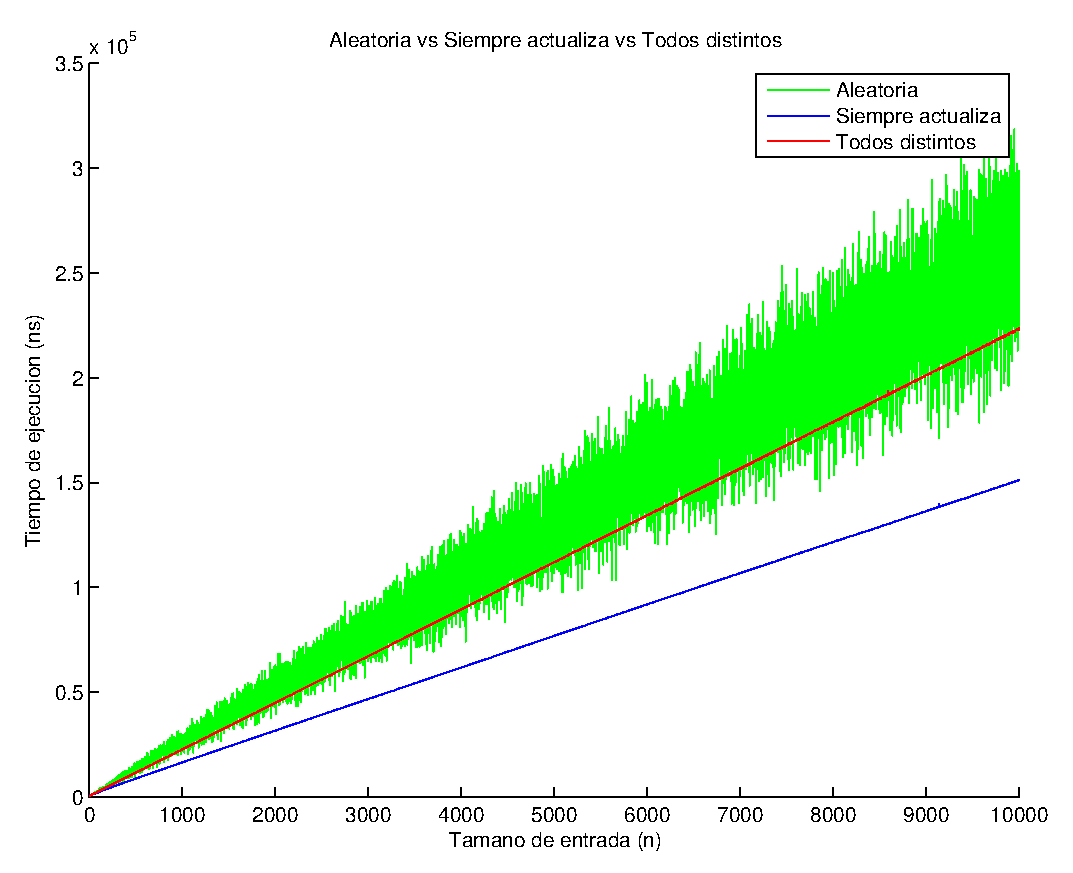
\includegraphics[width=0.6\linewidth]{problema1/graficos/problema1_ordenada_aleatoria_10000_vs_problema1_ordenada_siempre_actualiza_10000_vs_problema1_ordenada_todos_distintos_10000.eps}
    \end{center}
    \caption{Instancias aleatorias vs Siempre actualiza el máximo vs Todos días distintos. $1 \leq n \leq 10000$.}
    \label{fig:problema1-ordenadas-comparacion}
  \end{figure}

En el gráfico observamos un comportamiento lineal para los dos tipos de instancias particulares, y utilizando una técnica similar a la de la figura \ref{fig:problema1-aleatoria-10000}, lado derecho, concluímos lo mismo para las instancias aleatorias. Es decir, el ciclo presenta un costo temporal proporcional a la cantidad de camiones en la entrada. Adicionalmente, se observa que las instancias promedio consumen en general más tiempo que las instancias particulares generadas a modo comparativo.

% Curiosamente, ``siempre actualiza'' es mejor que ``Todos distintos''. Investigamos y llegamos a la conclusión que esto se debe a como creamos las instancias de entrada. Las creamos siguiendo la siguiente secuencia:

% % % % 

% Como tiene números repetidos, el algoritmo saltea varias iteraciones en la parte del siguiente \emph{for}.

% ^^^^^ esto creo que está mal. como tiene repetidos entonces se saltea todo el cuerpo del ciclo, no influye en este for

% \begin{verbatim}
%   for (; (j < e.cant_dias) && (dias[j] - dias[i] < e.cant_dias_inspeccion); ++j)
%       ;
% \end{verbatim}

% Por esta razón, termina siendo mejor que el de ``Todos distintos''.
